%%####################################################################
%    Copyright @ 2007 Andreas Frieß (Friess)
%    Permission is granted to copy, distribute and/or modify this document
%    under the terms of the GNU Free Documentation License, Version 1.2
%    or any later version published by the Free Software Foundation;
%    with no Invariant Sections, no Front-Cover Texts, and no Back-Cover Texts.
%    A copy of the license is included in the section entitled ``GNU
%    Free Documentation License''.
%%####################################################################
% Created: 20.01.2008
% @cvs($Date: $)
% @cvs($Rev: $)
% @cvs($Author: af0815 $)
% @cvs($URL: $)
%%####################################################################
\subsection[Projektschablonen]{Projektschablonen}
\subsubsection{Beschreibung}
Projektschablonen sind Vorlagen für öfters verwendete Projekte. Das Komponente "`projekttemplates"' hilft bei der Verwendung von Schablonen\footnote{auch Vorlagen genannt}. Als Vorbereitung muß man die Komponente installieren. 
\parpic[sl][r]{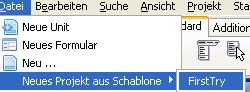
\includegraphics[width=0.3\textwidth]{Kapitel/ide/pics/PrjTempl01}}\label{fig:ProjectTempl01}Nach der Erstellung ist das Menü "`Werkzeuge"' um den Eintrag "`Optionen für Projektschablonen"' erweitert. Mit Hilfe dieses Menüpunktes kann man das Basis Verzeichnis für die Schablonen einstellen. \parpic[sr][l]{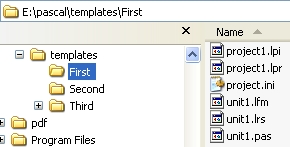
\includegraphics[width=0.3\textwidth]{Kapitel/ide/pics/PrjTempl02}}\label{fig:ProjectTempl02}Die Schablonen selbst befinden sich dann in den Unterverzeichnissen. Weiters wird auch das Menü "`Datei"' um den Eintrag "`Neues Projekt aus Schablone"' erweitert. Zusätzlich ist auch der "`Datei Neu .."' Dialog entsprechend erweitert.

Jede Schablone liegt in einem eigenen Unterverzeichnis und kann selbst weitere Unterverzeichnisse enthalten. Diese Struktur wird beim Erstellen eines neuen Projektes mittels Schablonen übertragen\footnote{Es mir in der derzeitigen Version Lazarus 0.9.25 svn 13811 nicht geglückt das die Unterverzeichnisse kopiert werden}.

Die Steuerung der Vorlagen erfolgt durch die Datei "`project.ini"'. Diese Datei ist im "`ini"' Format aufgebaut und es befinden sich derzeit zwei Sektionen darinnen. In der ersten Sektion mit dem Namen "`[Variables]"' befinden sich die Variablen\footnote{Platzhalter, veränderbare Teile}. Als Voreinstellung selbst gibt es zwei vordefinierte Variablen die die Ersetzungsroutine selbst kennt und die nicht definiert werden müssen.
\begin{description}
	\item[ProjDir]Das Verzeichnis, in welches das neue Projekt erzeugt wird
	\item[ProjName]Der Name des neuen Projektes
\end{description}
\parpic[sl][r]{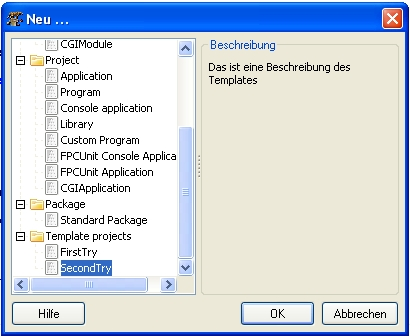
\includegraphics[width=0.4\textwidth]{Kapitel/ide/pics/PrjTempl04}}\label{fig:ProjectTempl04}Weitere Variablen, müssen in der Sektion "`[Variables]"' in der folgenden Form definiert werden. Zuerst kommt der Variablenname, dann das Gleichheitszeichen und zum Schluß eine Beschreibung, welcher in der Eingabemaske auf scheinen wird.
Während des kopierens können Ersetzungen durchgeführt werden. Das Kennzeichen für diese Ersetzung ist \_\_VARNAME\_\_\footnote{Wurde gegenüber der Beschreibung im README.txt offenbar geändert - war \$(VARNAME)}. Diese Zeichnenfolge wird durch den Inhalt der Variablen ersetzt. Die Bezeichnung "`VARNAME"' ist durch den Namen der Variable zu ersetzen. Die Ersetzung wird beim Kopieren in das neue Projekt sowohl in den Dateinamen gemacht, als auch innerhalb der Dateien. 

Die zweite Sektion beschäftigt sich mit dem beschreiben des Projektes selbst. Die Sektion "`[Project]"' beinhaltet folgende Informationen zum Projekt, wobei der Namen, Author und die Beschreibung in Datei-Neu Dialog von Lazarus angezeigt wird.
\begin{description}
	\item[Name]Namen der Vorlage
	\item[Author]Author der Vorlage
	\item[Description]Kurze Beschreibung der Vorlage, maximal einzeilig
	\item[Recurse] Ob in Unterverzeichnis hineinrekusiert\footnote{funktioniert ?!} werden soll (0=Nein, 1=Ja)
	\item[Exclude]Durch Komma getrennte Liste, welche Dateien nicht für die Ersetzung verwendet werden sollen
\end{description}	
Ist in dem Verzeichnis eine Datei mit dem Namen "`description.txt"', so wird der Inhalt der Datei als Beschreibung verwendet.

\subsubsection{Beispiel}
Als Beispiel habe ich ein vorhandenes einfaches Projekt im Vorlagen Verzeichnis abgespeichert. Weiter kommt in diese Verzeichnis eine "`project.ini"' Datei mit folgen Inhalt hinein
\begin{verbatim}
[Variables]
VarName1= Dateiname fuer das Hauptformular
[Project]
Name=SecondTry
Author= Nobody
Description= Test template 1
Recurse= 0
Exclude=
\end{verbatim}
\parpic[sr][l]{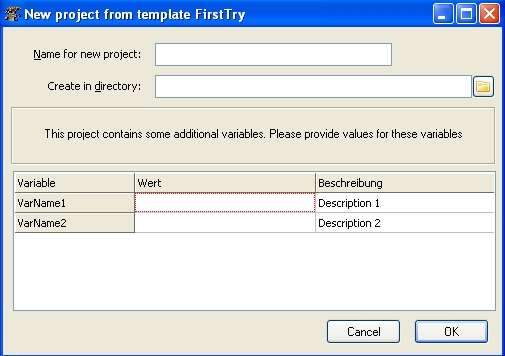
\includegraphics[width=0.3\textwidth]{Kapitel/ide/pics/PrjTempl05}}\label{fig:ProjectTempl05}
In der ersten Eingabezeile wird der Dateiname des Projektes eingegeben, er ist in der nicht sichtbaren Variablen "`ProjName"' dann vorhanden. In der zweiten Zeile gibt man den Pfad, wohin die Dateien aus den Vorlagen kopiert werden sollen an. Das kann entweder durch Direkteingabe erfolgen oder über den Dateidialog, den man rechts neben der Eingabezeile aufrufen kann. Darunter befindet sich dann die Eigabemaske für die frei (in der "`project.ini"') definierbaren Variablen. Der ausgefüllte Inhalt der Variablen ersetzt dann beim kopieren die Platzhalter.

Heisst also eine Datei im Templateverzeichnis zum Beispiel \textit{\_\_VarName1\_\_.pas} und bei der Variablen wird "`myform"' festgelegt, so wird die Datei als \textit{myform.pas} in das Zielverzeichnis kopiert. Ebenso verhält es sich mit Variablen (nicht verwechseln mit Variablen innerhalb von Lazarus), die beim kopieren ebenso durch die Werte ersetzt werden. 

Wird der Dialog jetzt bestätigt, so wird die Kopieraktion durchgeführt und Lazarus öffnet das neue Projekt.

\verb|Version: $ $ |\footnote{ Autor: Andreas Frieß\\Lizenz: GFDL}